\documentclass{report} % //TODO find why latex gives errors for report and using textsc!
\usepackage{fancyhdr}
\usepackage{graphicx}
\usepackage{amsmath}
\usepackage[margin=1in]{geometry}

\graphicspath{{./Pictures/}}

\title{CEE 442 Calculations Package - Beams}
\author{Anthony Le}
 
\newtheorem{exmp}{Example}
\newtheorem{exrc}{Excersize}
\newtheorem{proof}{Proof}
\newtheorem{defn}{Definition}


\begin{document}

\pagestyle{fancy}
\fancyhead{}
\fancyhead[R]{CEE 442 SD Calculations Package}
\fancyhead[L]{SCHALT Structural}



\section*{Preliminary Structural Calculations}
\subsection*{Gravity System Design}
\subsubsection*{Sizing Roof Beams (Covering Gridlines A6-B6)}

\begin{center}
    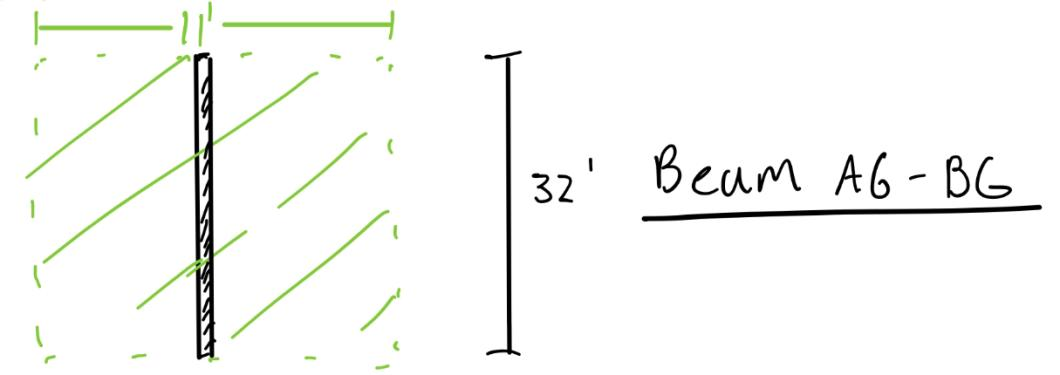
\includegraphics[scale=0.25]{RoofBeams_A6_B6}
\end{center}

Given:
\begin{equation*}
    \begin{aligned}
        &LL = 100psf &\quad SDL = 55.83psf \\
        &W_{trib} = 11ft &\quad L_b = 32ft 
    \end{aligned}
\end{equation*}
Find: 
\begin{enumerate}
    \item $M_u$
    \item Select W-Section using AISC A360-16 Table 3-10
\end{enumerate}
Solve:
\begin{center}
    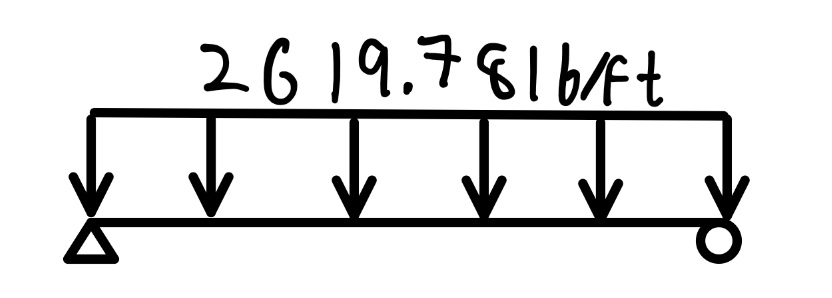
\includegraphics[scale=0.15]{RoofBeams_A6_B6_Loads}
\end{center}
\begin{enumerate}
    \item Controlling LRFD Load Combo:
        \begin{equation*}
            \begin{aligned}
                1.4D + 1.6l &= 1.4(55.83psf) + 1.6(100psf) \\
                            &= 238.16psf 
            \end{aligned}
        \end{equation*}
        \item Finding LRFD Factored Distributed Load, $W_u$:
        \begin{equation*}
            \begin{aligned}
                W_u &= (238.16psf)(11ft) \\
                W_u &= 2619.78 lb/ft 
            \end{aligned}
        \end{equation*}
    \item Finding Reaction Forces:
        \begin{equation*}
            \begin{aligned}
                A_y = B_y &= \frac{wL}{2} \\
                        &= \frac{(2619.78 lb/ft)(32 ft)}{2} \\
                A_y = B_y &= 41.92K
            \end{aligned}
        \end{equation*}
    \item Finding LRFD Factored Moment, $M_u$:
        \begin{equation*}
            \begin{aligned}
                M_u &= \frac{wL^2}{8} \\
                    &= \frac{(2619.78 lb/ft)(32 ft)^2}{8} \\
                M_u &= 335.33 K-ft
            \end{aligned}
        \end{equation*}
    \item Selecting W-Section:\\
    Assuming an unbraced length using $L_b$ = 32 ft from A360-16 Table 3-10, where:
        \begin{equation*}
            \begin{aligned}
                \Phi M_n \geq M_u \\
                \Phi M_n \geq 335.53 K-ft
            \end{aligned}
        \end{equation*}
\end{enumerate}
\begin{center}
    \fbox{Select W18X86}
\end{center}

\newpage
\subsubsection*{Sizing Roof Girders (Covering Gridlines B6-B7)}

Given:\footnote{Note that the applied forces P were calculated using the reaction of roof beams A6-B6 and the self-weight of the W18X86 beam.}
\begin{equation*}
    \begin{aligned}
        &P = 44.67K &\quad L = 33ft \\%41.92 + \frac{86lb/ft * 32ft}{2} //TODO - Clarify with Leo and Caitlin how they got their P values?
        &a = 11ft 
    \end{aligned}
\end{equation*}
Find: %//TODO - I'm a little unsure about why we're finding the required moment of inertia to select the section based off of the deflection here!
\begin{enumerate}
    \item $L/360$
    \item $M_{max}$
    \item $\Delta _{max}$
    \item $I_{required}$
    \item Select W-Section using AISC A360-16 Table 6-2
\end{enumerate}
Solve:

\begin{center}
    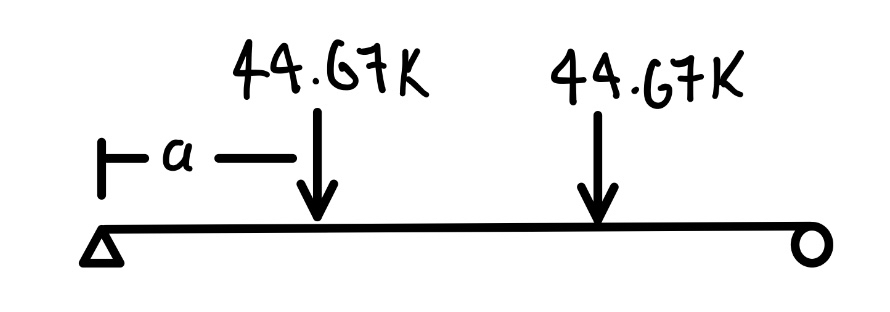
\includegraphics[scale=0.25]{RoofGirder_B6_B7_Loads}
\end{center}

\begin{enumerate}
    \item Finding $L/360$
        \begin{equation*}
            \begin{aligned}
                \Delta _{required} &= L/360 \\
                            &= (33ft * 12in)/360\\
                \Delta _{required} &= 1.10in    
            \end{aligned}
        \end{equation*}
    \item Finding $M_{max}$
        \begin{equation*}
            \begin{aligned}
                M_{max} &= P * a \\
                        &= 44.67K * (11ft) \\  %//TODO - How did Leo get a number for P? He doesn't make it clear in the beginning
                        &= 163.79 K-ft
            \end{aligned}
        \end{equation*} 
    \item Finding $\Delta _{max}$
        \begin{equation*}
            \begin{aligned}
                \Delta _{max} &= \frac{Pa}{24EI} * (3L^2-4a^2)\\ %//TODO - How did Leo get a number for I? He doesn't make it clear in the beginning
                        &= \frac{44.67K * 11ft * 12in}{24 * 29000ksi * 1330in^4} * (3(33ft * 12in)^2-4(11ft * 12in)^2) \\
                \Delta _{max} &= 2.01in    
            \end{aligned}
        \end{equation*}
    \item Finding $I_{required}$
        \begin{equation*}
            \begin{aligned}
                \Delta _{max} &> \Delta _{required} \\
                2.01 &> 1.10 \\
            \end{aligned}
        \end{equation*}
        Since $\Delta _{max} > \Delta _{required}$, we'll set $\Delta _{max} = \Delta _{required}$ and solve for I. Rearranging the equation and solving, we get:
        \begin{equation*}
            \begin{aligned}
                I_{required} = 2450in^4
            \end{aligned}
        \end{equation*}
    \item Selecting W-Section using AISC A360-16 Table 6-2 \\
    Assuming $L_b = 32ft$ from A360-16 Table 6-2 where:
        \begin{equation*}
            \begin{aligned}
                I_{required} = 2450in^4
            \end{aligned}
        \end{equation*}
\end{enumerate}
\begin{center}
    \fbox{W27X84}
\end{center}
Loading girder as simple beam with two equal concentrated load symmetrically placed  

\newpage
\subsubsection*{Sizing Roof Girders (Covering Gridlines A5-A6)}
Given:
\begin{equation*}
    \begin{aligned}
        &LL = 20psf \quad &SDL = 57.3psf \\
        &L_b = 33ft \quad &W_{trib} = 16ft \\
    \end{aligned}
\end{equation*}
Find:
\begin{enumerate}
    \item $M_u$
    \item Select W-Section using AISC A360-16 Table 3-10
\end{enumerate}
Solve:
\begin{enumerate}
    \item Finding LRFD psf with Controlling Load Combo:
        \begin{equation*}
            \begin{aligned}
                &1.4L + 1.6L \\ 
                \rightarrow &1.4(57.3) + 1.6(20) \\
                &=112.22psf\\   
            \end{aligned}
        \end{equation*}
    \item Finding LRFD Factored Distributed Load, $W_u$:
        \begin{equation*}
            \begin{aligned}
                W_u &= (112.22psf)(16ft) \\
                W_u &= 1745.52 lb/ft
            \end{aligned}
        \end{equation*}
    \item Finding Reaction Forces:
        \begin{equation*}
            \begin{aligned}
                A_y = B_y &= \frac{wL}{2} \\
                        &= \frac{(1745.52 lb/ft)(33 ft)}{2} \\
                A_y = B_y &= 29.636K
            \end{aligned}
        \end{equation*}
    \item Finding LRFD Factored Moment, $M_u$:
        \begin{equation*}
            \begin{aligned}
                M_u &= \frac{wL^2}{8} \\
                    &= \frac{(1745.52 lb/ft)(33 ft)^2}{8} \\
                M_u &= 244.42 K-ft
            \end{aligned}
        \end{equation*}
    \item Selecting W-Section:\\
        Assuming an unbraced length using $L_b$ = 33 ft from A360-16 Table 3-10, where:
            \begin{equation*}
                \begin{aligned}
                    \Phi M_n \geq M_u \\
                    \Phi M_n \geq 244.42 K-ft
                \end{aligned}
            \end{equation*}
            \begin{center}
                \fbox{Select W12X65}
            \end{center}
    \item Deflection Checks: \\
        Loading the girder with two equal concentrated load symmetrically with uniform distributed load:
        \begin{enumerate}
            \item Finding Self Weight Distributed Load
                \begin{equation*}
                    \begin{aligned}
                        P_{self} &= (86lb/ft)(32ft) \\ %//TODO - isn't this length of 32 ft supposed to be 33 ft?
                        P_{self} &= 2752lbs
                    \end{aligned}
                \end{equation*}
            \item Finding Cladding Distributed Load
                \begin{equation*}
                    \begin{aligned}
                        P_{cladding} &= (16psf)(295.5ft^2) \\ %//TODO - Shouldn't this be supposed to be 295.5*2 ft2 since we're spanning 33, not 16.5ft
                        P_{cladding} &= 4728lbs 
                    \end{aligned}
                \end{equation*}
            \item Finding $M_{max}$ 
                \begin{equation*}
                    \begin{aligned}
                        M_{max} &= P * a \\
                                &= 47.28K * (11ft * 12in) \\  %//TODO - How did Leo get a number for P? He doesn't make it clear in the beginning
                                &= 520.08 K-ft
                    \end{aligned}
                \end{equation*} 
        \item Finding $\Delta _{required}$
            \begin{equation*}
                \begin{aligned}
                    \Delta _{required} &= L/360 \\
                                &= (33ft * 12in)/360\\
                    \Delta _{required} &= 1.10in    
                \end{aligned}
            \end{equation*} 
        \item Finding $\Delta _{max}$
            \begin{equation*}
                \begin{aligned}
                    \Delta _{max} &= \frac{Pa}{24EI} * (3L^2-4a^2)\\ %//TODO - How did Leo get a number for I? He doesn't make it clear in the beginning
                            &= \frac{47.28K * 11ft * 12in}{24 * 29000ksi * 533in^4} * (3(33ft * 12in)^2-4(11ft * 12in)^2) \\
                    \Delta _{max} &= 1.06in \\
                    \Delta _{max} &< \Delta _{required}, \text{Passes deflection checks}    
                \end{aligned}
            \end{equation*}
        \end{enumerate}
\end{enumerate}

\newpage
\subsubsection*{Sizing Roof Interior Columns (Covering Gridline B7)}
\begin{center}
    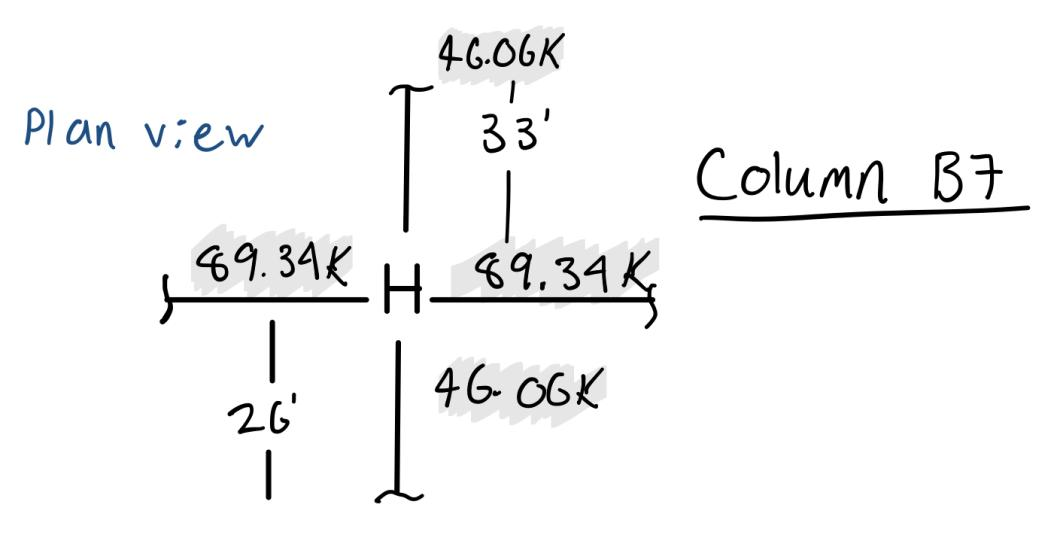
\includegraphics[scale=0.25]{RoofColumn_B7}
\end{center}
Given:
\begin{equation*}
    \begin{aligned}
        &P_x = 89.34K \quad &P_y = 46.06K \\
        &L_{\text{B7 to A7}} = 33ft \quad &L_{\text{B7 to C7}} = 26ft \\
        &\text{Assume Lc/r = 50} \quad &L_{cx} = 15ft
    \end{aligned}
\end{equation*}
Find:
\begin{enumerate}
    \item $A_{required}$
    \item $P_u$
    \item $P_n$
    \item Select W-Section using AISC A360-16 Table 4-1a
\end{enumerate}
Solve:
\begin{center}
    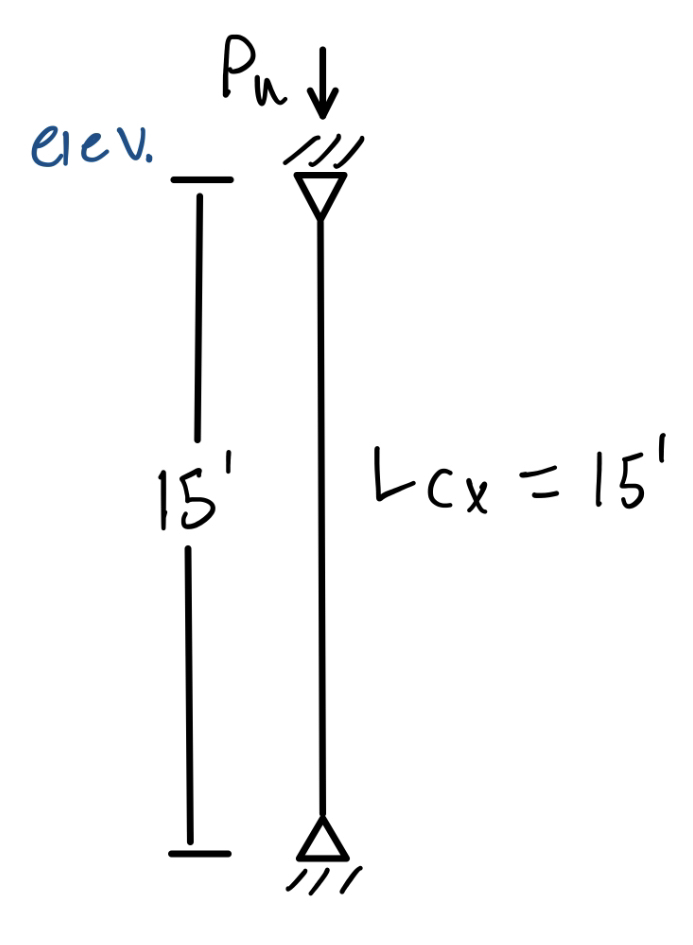
\includegraphics[scale=0.15]{RoofColumn_B7_Loads}
\end{center}
\begin{enumerate}
    \item Finding Axial Loading on Column:
        \begin{equation*}
            \begin{aligned}
                P_u &= 2(P_x) + 2(P_y) \\
                    &= 2(89.34K) + 2(46.06K) \\
                P_u &= 270.8K  
            \end{aligned}
        \end{equation*}
    \item Selecting W-Section:\\
        Assuming an unbraced length using $L_c/r$ = 50 and selecting from A360-16 Table 4-1a:
            \begin{center}
                \fbox{Select W14X48, $A_{g,provided} = 14.1in^2$}
            \end{center}    
\end{enumerate}
Buckling Failure Checks:
\begin{enumerate}
    \item Finding Elastic Buckling Stress, $F_e$:
        \begin{equation*}
            \begin{aligned}
                F_e &= \frac{\pi^2E}{(L_c/r)^2} \\
                F_e &= \frac{\pi^2*29000}{(50)^2} \\
                F_e &= 114.5K
            \end{aligned}
        \end{equation*}
    \item Finding slenderness ratio limit, $4.71\sqrt{E/F_y}$:
        \begin{equation*}
            \begin{aligned}
                4.71\sqrt{E/F_y} = 4.71\sqrt{29000Ksi/50ksi} = 113.43 
            \end{aligned}
        \end{equation*}
    \item Finding Critical Buckling Load, $F_{cr}$: \\
        Since $50 < 113.43$, we will have failure in buckling 
        \begin{equation*}
            \begin{aligned}
                F_{cr} &= F_y(0.658^{Fy/Fe}) \\
                        &= 50ksi * (0.658^{50ksi/114.5ksi}) \\
                        &= 41.65
            \end{aligned}
        \end{equation*}
    \item Checking if $A_{g,required}$ exceeds $A_{g,provided}$:
        \begin{equation*}
            \begin{aligned}
                P_u &\leq 0.9F_{cr}A_g \\
                266.4 &\leq 0.9(41.6ksi)(A_{g,required}) \\
                A_{g,required} &\geq 7.12 \\
                A_{g,provided} &\geq A_{g,required} \\
                14 &\geq 7.12 
            \end{aligned}
        \end{equation*}
        Selected section passes buckling and slenderness checks.
\end{enumerate}

\newpage
\subsubsection*{Sizing Roof Exterior Columns (Covering Gridline A8)}
\begin{center}
    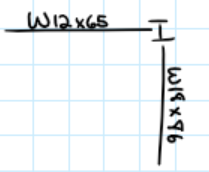
\includegraphics[scale=1.25]{RoofColumn_A8}
\end{center}
Given:
\begin{equation*}
    \begin{aligned}
        &P_x = 54.31K \quad &P_y = 23.5K \\
        &\text{Assume Lc/r = 50} \quad &L_{cx} = 15ft
    \end{aligned}
\end{equation*}
Find:
\begin{enumerate}
    \item $A_{required}$
    \item $P_u$
    \item $P_n$
    \item Select W-Section using AISC A360-16 Table 4-1a
\end{enumerate}
Solve:
\begin{center}
    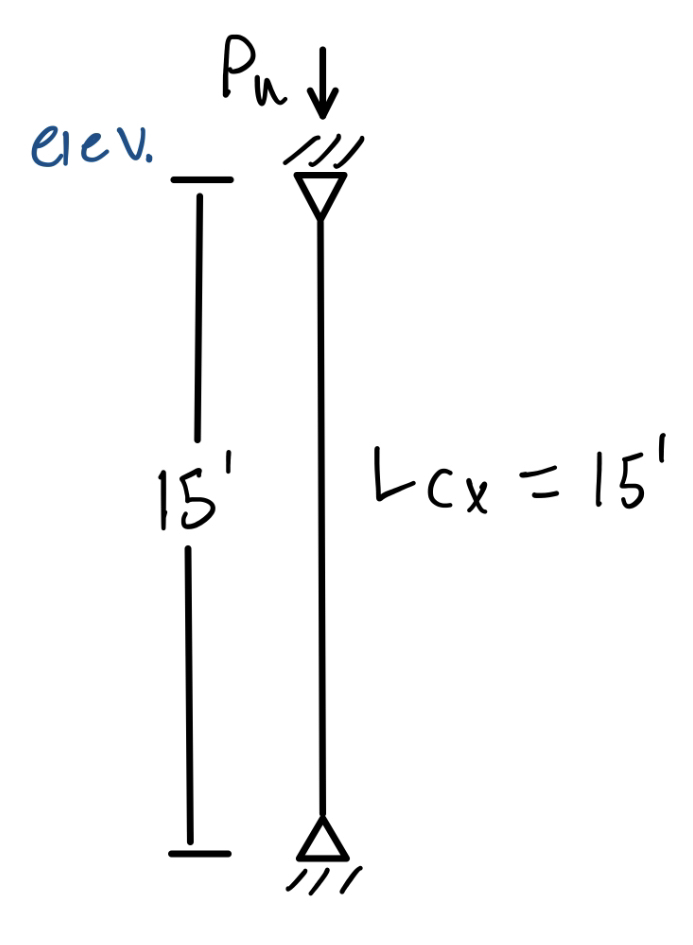
\includegraphics[scale=0.15]{RoofColumn_B7_Loads}
\end{center}
\begin{enumerate}
    \item Finding Axial Loading on Column:
        \begin{equation*}
            \begin{aligned}
                P_u &= P_x + P_y \\
                    &= 54.31 + 23.5 \\
                P_u &= 77.8K  
            \end{aligned}
        \end{equation*}
    \item Selecting W-Section:\\
        Assuming an unbraced length using $L_c/r$ = 50 and selecting from A360-16 Table 4-1a:
            \begin{center}
                \fbox{Select W14X26, $A_{g,provided} = 7.69$}
            \end{center}    
\end{enumerate}
Buckling Failure Checks:
\begin{enumerate}
    \item Finding Elastic Buckling Stress, $F_e$:
        \begin{equation*}
            \begin{aligned}
                F_e &= \frac{\pi^2E}{(L_c/r)^2} \\
                F_e &= \frac{\pi^2*29000}{(50)^2} \\
                F_e &= 114.5K
            \end{aligned}
        \end{equation*}
    \item Finding slenderness ratio limit, $4.71\sqrt{E/F_y}$:
        \begin{equation*}
            \begin{aligned}
                4.71\sqrt{E/F_y} = 4.71\sqrt{29000Ksi/50ksi} = 113.43 
            \end{aligned}
        \end{equation*}
    \item Finding Critical Buckling Load, $F_{cr}$: \\
        Since $50 < 113.43$, we will have failure in buckling 
        \begin{equation*}
            \begin{aligned}
                F_{cr} &= F_y(0.658^{Fy/Fe}) \\
                        &= 50ksi * (0.658^{50ksi/114.5ksi}) \\
                        &= 41.65
            \end{aligned}
        \end{equation*}
    \item Checking if $A_{g,required}$ exceeds $A_{g,provided}$:
        \begin{equation*}
            \begin{aligned}
                P_u &\leq 0.9F_{cr}A_g \\
                77.8 &\leq 0.9(41.6ksi)(A_{g,required}) \\
                A_{g,required} &\geq 2.06 \\
                A_{g,provided} &\geq A_{g,required} \\
                7.696 &\geq 2.06 
            \end{aligned}
        \end{equation*}
        Selected section passes buckling and slenderness checks.
\end{enumerate}

\subsection*{Lateral System Design}
\subsubsection*{Sizing Roof Lateral System Braces (Covering Gridlines B3-C3)}
\begin{center}
    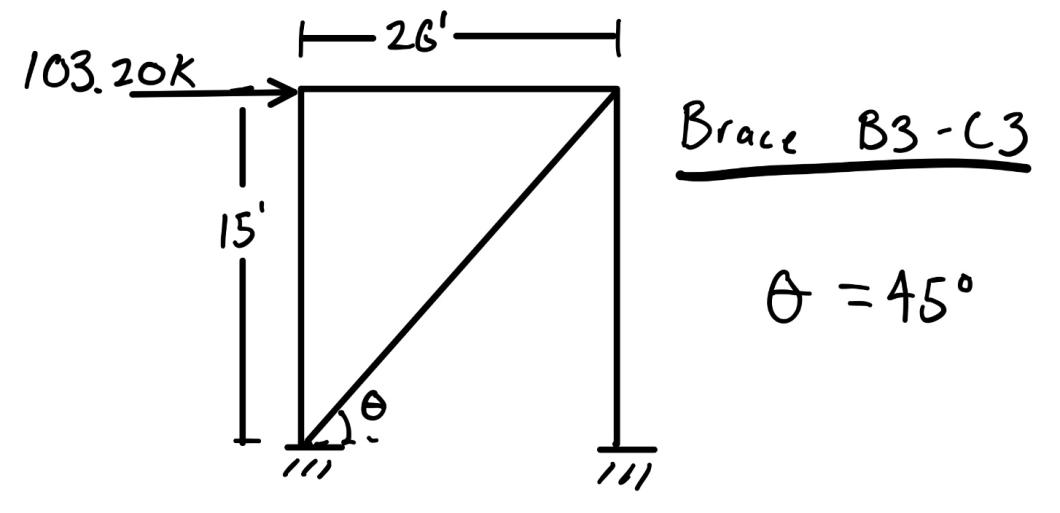
\includegraphics[scale=0.15]{RoofLateralSystem_B3_C3}
\end{center}
Given:
\begin{equation*}
    \begin{aligned}
        &W = 26ft &\quad H = 15ft \\
        &\Phi P_n = 103.20K &\quad \Theta = 45
    \end{aligned}
\end{equation*}
Find: 
\begin{enumerate}
    \item $A_sc$
    \item Select BRBF Section from CoreBrace BRB Reference Guide
\end{enumerate}
Solve:
\begin{enumerate}
    \item Finding $P_{max}$:
        \begin{equation*}
            \begin{aligned}
                P_{max} &= P \cos \Theta \\
                        &= 103.20\cos(45) \\
                P_{max} &= 72.97K
            \end{aligned}
        \end{equation*}
    \item Finding $A_{sc}$
        \begin{equation*}
            \begin{aligned}
                A_{sc} &= \frac{P_{max}}{F_{y,min}} \\
                       &= \frac{72.97K}{36Ksi} \\
                A_{sc} &= 2.03in^2 
            \end{aligned}
        \end{equation*}
        \begin{center}
            \fbox{Select t8(203.2)(3in$^2$)}
        \end{center}
\end{enumerate}

\subsubsection*{Sizing Roof Lateral System Column (Covering Gridlines B3-C3)}
\begin{center}
    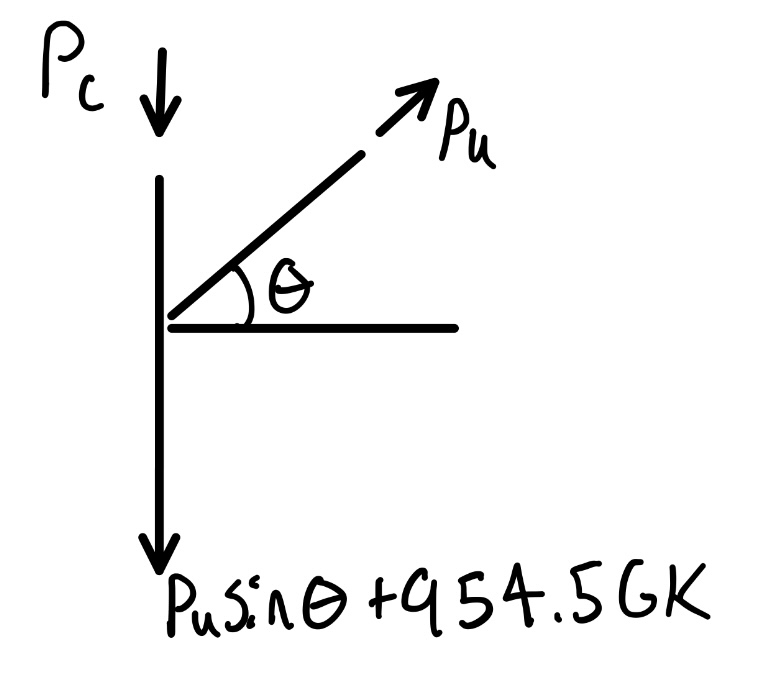
\includegraphics[scale=0.15]{RoofLateralSystem_B3_C3_Loads}
\end{center}
Given:
\begin{equation*}
    \begin{aligned}
        &B = 1.1 &\quad W = 1.36 \\
        &\Phi P_n = 103.20K &\quad \Theta = 45 \\
        &Factored Load = 238.16psf &\quad P_{above} = 270.8K
    \end{aligned}
\end{equation*}
Find: 
\begin{enumerate}
    \item $P_c$
    \item Select W-Section using AISC A360-16 Table 4-1a
\end{enumerate}
Solve:
\begin{center}
    \includegraphics[scale=0.15]{RoofLateralSYstem_B3_C3_Loads}
\end{center}
\begin{enumerate}
    \item Finding $P_u$:
        \begin{equation*}
            \begin{aligned}
                P_u = wA_{sc}F_{y,max} (T) \\
                P_u = BwA_{sc}F_{y,max} 
            \end{aligned}
        \end{equation*}
    \item Finding Tributary Area, $A_t$
        \begin{equation*}
            \begin{aligned}
                A_t &= 33ft*(26/2ft+32/2) \\
                A_t &= 957ft^2
            \end{aligned}
        \end{equation*}
    \item Finding $P_c$
        \begin{equation*}
            \begin{aligned}
                P_c &= P_{above} + \text{Factored Load} * A_t \\ 
                P_c &= 270.8K + 238.16psf(957ft^2)/1000 \\
                P_c &= 954.56K
            \end{aligned}
        \end{equation*}
    \item Select W-Section using AISC A360-16 Table 4-1a
        \begin{center}
            \fbox{Select W14X99, $\Phi P_n = 1100K$}
        \end{center}
\end{enumerate}
\end{document}

